\documentclass[12pt,a4paper]{article}
\usepackage[utf8]{inputenc}

\usepackage{amsmath}
\usepackage{amsfonts}
\usepackage{amssymb}
\usepackage{graphicx}
\usepackage{color}
\usepackage{enumerate}
\usepackage{lineno}
\usepackage{listings} 
\definecolor{lightgrey}{rgb}{0.90,0.90,0.90}
\lstset{language=Java, backgroundcolor=\color{lightgrey},  numbersep=5pt, tabsize=3}

\setlength{\parindent}{0em}
\setlength{\parskip}{0.5em}

\title{Lösungsstrategien für NP-schwere Probleme\\Blatt 5}
\author{
		Jakob Rieck\\
		\small{6423721}
	\and
		Konstantin Kobs\\
		\small{6414943}
	\and
		Thomas Maier\\
		\small{6319878}
	\and
		Tom Petersen\\
		\small{6359640}
}
\date{Abgabe zum 23.05.16}


\begin{document}

\maketitle

\section*{Aufgabe 1}

 \begin{enumerate}[a)]

 	\item 
 	\begin{figure}[ht]
 		\centering
 		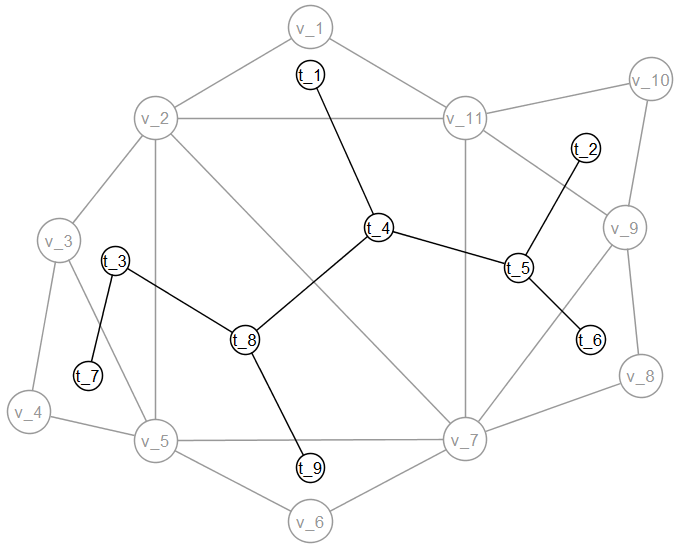
\includegraphics[scale=0.5]{Baumzerlegung.png}
 		\caption{Baumzerlegung}
 		\label{baumzerlegung1a}
 	\end{figure}
 	
 	Figure \ref{baumzerlegung1a} zeigt die gewünschte  Baumzerlegung $(T,\{V_t:t\in T \})$, wobei $T= \{t_i : 1 \le i \le 9\}$ und $V_{t_1}=\{v_1,v_2,v_{11}\}$, $V_{t_2}=\{v_9,v_{10},v_{11}\}$, $V_{t_3}=\{v_2,v_3,v_5\}$, $V_{t_4}=\{v_2,v_{11},v_7\}$, $V_{t_5}=\{v_7,v_9,v_{11}\}$, $V_{t_6}=\{v_7,v_8,v_9\}$, $V_{t_7}=\{v_3,v_4,v_5\}$, $V_{t_8}=\{v_2,v_5,v_7\}$, $V_{t_9}=\{v_5,v_6,v_7\}$ gilt.
 	
	\item Das Ziel des Algorithmus ist es, aus jedem Dreieck in dem Graphen einen Knoten $t \in T$ zu finden, so dass $|V_t| = 3$ gilt. \textbf{Eingabe:} Ein triangulierter Kreisgraph $G=(V,E)$. \\
	Nun betrachten wir zwei Fälle: \\
	\\
	\textit{1. Fall:} Der Eingabegraph $G$ besteht nur aus drei Knoten. In diesem Fall ist $T$ Einelementig und $V_t=V$ für $t\in T$. \\
	\\
	\textit{2. Fall:} Der Eingabegraph $G$ besteht aus mehr als drei Knoten. In diesem Fall werden die äußeren Dreiecke des Graphen $G$ betrachtet. Ein äußeres Dreieck besitzt einen (in diesem Fall genau einen) Knoten $v$ mit Grad = 2. $v$ bildet mit seinen beiden Nachbarknoten ein äußeres Dreieck. Der Algorithmus sucht also in dem Graphen $G$ einen Knoten $v$, dessen Grad = $2$ ist. Für dieses $v$ wird ein Knoten $t$ und die Menge $V_t = {v} \cup {Nachbarn(v)}$ in die Baumzerlegung hinzugefügt. Anschließend wird der Knoten $v$ aus $G$ entfernt und der nächste Knoten mit Grad = $2$ gesucht.     
\end{enumerate}

\section*{Aufgabe 2}

\begin{enumerate}[a)] 
	
	\item ...
\end{enumerate} 

\end{document}